\graphicspath{{chapters/images/10}}
\chapter{Ancient DNA}

\section{Iceman's history}
Thirty years ago Erika and Helmut Simon, while hiking on the Italian - Austrian border, stumbled over a skeleton half sticking in the ice.
The hut owner called the police and the dead body was recovered (believing it was a recent death, no archeological retrieval).
Luckily, many photos were taking during the excavation, allowing to keep track of more details.
After some days, an archeologist was called and established that the body had to be at least $4000$ years old.
The mummy is now conserved in Bolzano under specific conditions; the body, which is around $50 kg$, is losing weight over time, so spraying and temperature/humidity modifications are required to ensure a correct conservation.

	\subsection{Iceman's equipment}
	The Iceman’s equipment is composed by tools and clothes.
	61 tattoos were identified all over the body with the help of multispectral photography, mainly lines and crosses.
	Most likely this was a treatment for pain, stitch tattoos.
	It was initially thought that the Iceman died for the cold.
	Interestingly, in the stomach traces of hop hornbeam pollen were retrieved.
	This particular pollen is only present when hop hornbeam is in bloom, so Ötzi died in late spring.
	In 2001, by examining radiological analyses, it was possible to discover an arrowhead: the Iceman was murdered, a new 3D reconstruction proved that the arrow injury was lethal.
	The Iceman tried to pull out the arrow, but the arrowhead remained in the shoulder – maybe he wanted to hide that he was injured.

	\subsection{\"Otzi life}
	Ötzi lived approx.
	3.300 BC and died at 40-50 years old.
	He suffered from mild osteoarthritis of new joints (probably due to mountain hiking), intestinal parasites and arteriosclerosis.
	The isotopic analysis confirmed that he grew and lived in Northern Italy.
	A lot of results came back in the last years, but many samples were lost.
	In 2007 the Institute for Mummies and the Iceman was built, focus on molecular analysis (especially DNA) and preservation.

\section{Ancient DNA analysis}
The first study ancient DNA study was performed on a museum quagga specimen, an extinct member of the horse family.
Svante Pääbo is famous for his research on Neanderthal genome: by analyzing genomes retrieved from mummies through histology and DNA analysis he was able to perform mitochondrial DNA extraction and cloning.
It was later seen that a long mitochondrial DNA stretch was a modern human DNA contamination, bringing awareness in the field of the risk of contamination.

	\subsection{Impact of NGS}
	Thanks to NGS and PCR, it is now possible to exactly discriminate ancient DNA from modern DNA (by paying attention to potential overlaps).
	After an organism dies, post-mortem degradation begins.
	We have differences in pH, enzyme degradation, obtaining highly fragmented biomolecules.
	If the conditions are right e.g. permafrost, we can still use 7000 years old DNA.
	Modern DNA can also degrade, we can find small fragments.
	Through new techniques we can perform shotgun sequencing (all DNA) in silico and distinguish modern from ancient on the basis of damage patterns.
	Cytosines tend to deaminate over time, the C to T change can be effectively measured.
	In ancient DNA, we have a higher substitution frequency (figure \ref{fig:ct}).

	\begin{figure}[h]
	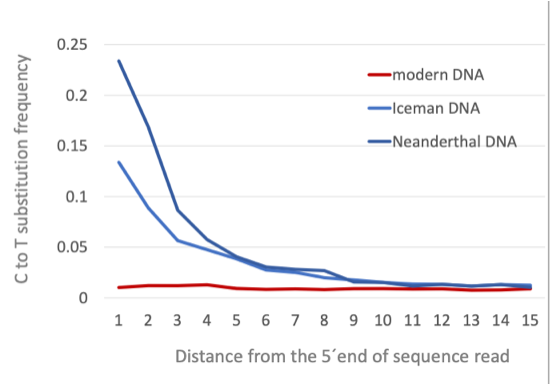
\includegraphics[width=0.7\textwidth]{ct.png}
	\caption{\label{fig:ct} C to T substitution frequency in modern, Iceman and Neanderthal DNA}
	\end{figure}

	Most of the ancient DNA is highly contaminated, and much depends on the conservation environment (we should protect samples from external DNA).
	For ancient DNA analysis, we extract the sample, build a DNA library and either perform shotgun sequencing or enrich for a specific site of interest.

\section{Iceman's genome}
While performing a metagenomic analysis of the Iceman’s shoelace leather, it was possible to identify the particular cattle species used for producing the leather, gaining insights into the animal sources of the Iceman’s Copper Age clothing.
The genetic analysis of the Iceman human genome started in 1994.

	\subsection{Genome analysis}
	After some unsuccessful attempts, it was possible to sequence the entire mitochondrial genome and nuclear genome.
	The Iceman genome project managed to over most of the genome ($>85\%$) with average coverage of $7x$ [SOLiD 4 sequencer, old machine].
	It was able to confirm authenticity and had a low level of contamination.
	Thanks to the project, it was possible to obtain data on pigmentation, SNP association indicates a high probability for brown eyes, light skin color and brown/blond hair, and clinical diseases: \"Otzi was  lactose intolerant, increased risk factor for cardiovascular disease (high common in other mummies, old lifestyle led to a higher risk).

	\subsection{Population genomics}
	Population genomics: project comparing a group of Early European farmers to modern European.
	Most of the skeleton samples clustered close to the Sardinian.
	This is probably due to an island effect.

\section{Iceman's metagenome}
The Iceman's metagenome was compared to 16s databases, finding a high abundance of Clostridia and Pseudomonas.
The third genus was Treponema, where most reads were assigned to T. denticola, belonging to a group of pathogens responsible for periodontitis (chronic inflammatory disease of the periodontium).
These oral flora bacteria are also involved in plaque formation.

	\subsection{Plaque analysis}
	BY applying PCR-based detection of red complex bacteria in Iceman’s mouth samples, it was possible to identify Treponema denticolsa and Porphyromonas gingivalis.
	Ancient dental calculus, present on top of the teeth, is an interesting plaque formation, which could be useful for many archeological studies (e.g. food traces, pathogens, human proteins).
	A diacronic sample set (different location and time origin) was used to study the dental calculus.
	A high abundance of the archea Methanovrevibacter was previously linked to ancient calculus.
	The study aimed at analyzing the diversity of archea in ancient calculus over time.
	All calculus samples contained reads assigned to the genus Methanovrevibacter and some had a very high abundance.
	Only one strain was linked to the known Methanovrevibacter, while the others unravelled new branches in the phylogeny – one linked to copper age, others to early middle age.
	There was a clear tendency in time for the diverse presence of different strains.
	Through functional analysis, it was seen that all the strains are involved in methanogenesis.
	To summarize, this study was able to perform de novo assembly on ancient dental calculus.
	There is a possible decline in Methanovrevibacter over time, but we lack modern calculus for comparison to fully assess it.

	\subsection{Iceman’s stomach}
	The completely filled stomach was not in its original anatomical position, it moved to the lung region.
	By sampling the stomach, it was possible to reconstruct diet and perform Helicobacter pylori diagnostics (figure \ref{fig:omics}.

	\begin{figure}
		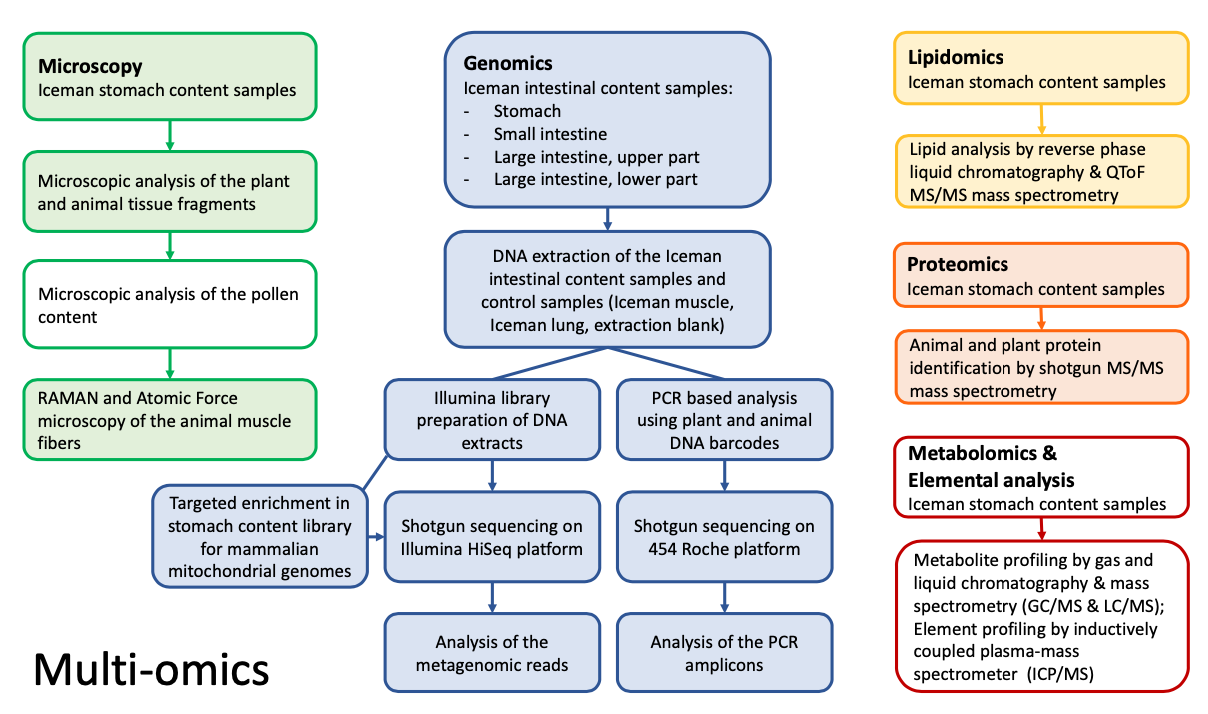
\includegraphics[width=1\textwidth]{multiomics.png}
		\caption{\label{fig:omics} Multi-omics analysis of the Iceman samples}
	\end{figure}

	The Iceman had an omnivorous diet: plants, muscle fibers with different length and breadth.
	The DNA-based analysis showed a high presence of background proteobacteria and firmicutes.
	Eukaryotic reads linked to diet are only 0.7\% to 0.2\%.
	Through them, it was possible to trace capra ibex reads and cerbus elaphus reads (last meals for the Iceman).
	Thanks to protein-based analysis, an animal diet was confirmed.
	For what concerns the plant diet, chloroplast genomes were traced – Poaceae reads traced to a monococcum wheat (cultivated) and Dennstaedtiaceae to Pteridium aquilinum, toxic herb (also consumed in Asia).
	The high hydrophobic property of the stomach content were studied in order to discriminate if fat derives from animals or plants, or dairy products.
	Initial histology highlighted the presence of adipose tissue, meat related.
	A lipid analysis was performed with HPLC-Chip/QTOF-MS, which discriminates fat types according to chain length; Ötzi TAG profile points towards ruminant meat and/or dairy products.
	By performing a comparative TAG profiling for meat and fat from ibex and red deer, milk and cheese from sheep and goat, it was seen that the Iceman had a high level of saturated fatty acids.

		\subsubsection{Summary}
		Ötzi had an omnivorous diet including wild meat, cereals and bracken.
		DNA- and Protein-based analysis indicate that the meal contained tissue of two different wild animals (red deer, ibex).
		High amount of lipids: TAG, DAG, cholesterol esters, phosphatidyl-cholines, sphingomyelins TAG profile matches that of mammalian tissues, especially fat from wild ruminants.
		No indication of dairy products consumption - Iceman could have been a shepherd or a migratory herder.
		RAMAN and AFM analysis of meat fibers reveal no indications for meat preparation with fire (cooked, fried/ roasted).
		Meat was most presumably air dried or smoked over the fire ( under 60°C).

\section{Helicobacter pylori}
Helicobacter pylori is a gram-negative bacterium, which infects $>50\%$ of humans globally.
It causes chronic gastritis, ulcers, adenocarcinoma.
It is transmitted predominantly vertically (intra-familial) and is usually acquired early in childhood causing a lifelong infection.
It is used as a marker for tracing human demographic events and recombines frequently.

	\subsection{Presence in the Iceman}
	H.pylori in the Iceman's stomach: usually H. pylori is studied through the histological analysis of the stomach mucosa (staining).
	Through PCR-based diagnostics, $\frac{2}{20}$ samples resulted to be PCR positive, but seemed to be a false positive.
	Through metagenomics, a decent number of unambiguous H. pylori DNA were retrieved in all gastrointestinal tract contents.
	The reads display a damage pattern typical of the ancient DNA.
	The distribution pattern of the DNA is coherent with the location, as most reads mapped to the stomach corpus.
	In order to overcome the background noise, RNA-based enrichment for H. pylori was performed.
	In this way we reduce diversity e.g. specific Iceman features, but we obtain a high enrichment effect (216-fold enrichment).
	The Iceman H. pylori reads map on $90\%$ of the reference genome (only one strain, 26695) with a 20-fold average coverage.
	Virulence factors indicate how severe an infection can be.
	CagA (cytotoxine-associated gene A) and VacA (vacuolating cytotoxin A) virulence factors were present in the Iceman, they provide a high probability of developing a severe disease form.
	To check whether the Iceman suffered from the disease, we would need to perform an histological exam (infeasible).
	Some proteins linked to infection were upregulated, suggesting the presence of the infection.

	\subsection{Genetic diversity of H. pylori}
	Studies on genetic variation showed that H. pylori diversity is highly structured.
	Looking at SNPs and flanking sites, we can sense the differences between European, Asian, African H. pylori strains.
	We can see a geographic pattern.
	Iceman’s strain belonged to a prehistoric European branch of hpAsia2 that is different from the modern hpAsia2 population from northern India.
	The distribution of hpAsia2 suggests it was widespread across Eurasia during the paleolithic and subsequently replaced by hpEurope.
	Despite the constant Middle Eastern immigration starting 10,000 BP (LGM) into Europe 5300 years ago, the replacement of ancient European hpAsia2 strains (like Ötzi’s) was not yet complete.
	These migrations were continuous, and occurred much more recently than previously thought.

	\subsection{Taxonomic profiling of the Iceman’s microbiome}
	The mummification was not fully finished in Ötzi’s corpse, the body was dehydrated and frozen and enzymes could not work.
	This is the main cause of high presence of Pseudomona and Clostridiae, involved in post-mortem processes (proteolytic breakdown of proteins, hydrolysis of fat and carbohydrates).
	The taxonomic profiling plus filtering indicates the presence of endogenous ancient gut bacteria.

	\subsection{Coprolite samples analysis}
	Ancient coprolite and gastric content samples were collected to get insights into the community composition of gut bacteria.
	A study focused on Mexican coprolite samples for caves, pre-colombian (660 to 1430 AD), established that H. pylori is less present in these samples with respect to the Iceman.
	The human DNA was linked to different sex and to genetic variation.
	The taxonomic composition shows high similarity to modern gut communities.

\section{Prevotella copri}
Prevotella copri is a frequently observed inhabitant of the human gut.
It aids in glucose tolerance but is responsible for rheumatoid arthritis and is abundant in HIV patients.
To extend the knowledge on its population structure and genetic diversity, a huge collection of modern gut samples from different sources was collected and analyzed.
A novel mapping based on a contig binning approach was applied along with a strict quality control.
Four different clades were identified with some country-specific sub-types.
A high prevalence and co-presence of multiple P. copri complex clades is typical in individuals from non-Westernized populations.
There is a considerably larger P. copri functional potential in non-Westernized populations e.g. distinct carbohydrate metabolism repertoires in the four clades.
P. copri diversity in ancient human gut contents resembles that of non-Westernised populations.
Clocking-based approach and dating methods can be used to see when the splits of certain clades happend e.g. humankind in Africa, then migration events carried Prevotella clades.
All this links to an interesting observation: there are indications for a loss of diversity throughout time, our ancestors had more diversity.
